\documentclass[aspectratio=169,11pt]{beamer}
\usepackage[T1]{fontenc}\usepackage{lmodern}\usepackage{booktabs}\usepackage{array}
\usepackage{tikz}\usetikzlibrary{arrows.meta,positioning,shapes.geometric}
\usepackage{xcolor}
\usepackage{booktabs}
\usepackage{tabularx}
\usepackage{array}
\usepackage[table]{xcolor}
\definecolor{NITNavy}{RGB}{18,42,76}\definecolor{NITBlue}{RGB}{39,91,145}\definecolor{NITLight}{RGB}{232,241,250}
\setbeamercolor{frametitle}{fg=NITNavy}\setbeamercolor{structure}{fg=NITBlue}\setbeamertemplate{navigation symbols}{}
\setbeamertemplate{footline}{\hfill\insertframenumber\hspace{0.5cm}\vspace{0.15cm}}

% \setbeamertemplate{frametitle}{
%     \vspace{.05cm}
%     \begin{beamercolorbox}
%         [wd=\paperwidth,sep=.08cm,leftskip=.55cm]
%         {frametitle}
%         \insertframetitle
%     \end{beamercolorbox}
%     \vspace{-.20cm}
%     \hspace{.55cm}
%     \rule{.91\paperwidth}{.6pt}
% }

\setbeamerfont{frametitle}{
    size=\large,
    series=\bfseries
}

\setbeamercolor{frametitle}{
    fg=NITNavy
}

\setbeamerfont{frametitle}{
    size=\large,
    series=\bfseries
}

\setbeamercolor{frametitle}{
    fg=white,
    bg=NITNavy
}

\setbeamertemplate{frametitle}{
    \vskip 0.15cm

    \begin{beamercolorbox}[
        wd=\paperwidth,
        ht=0.85cm,
        dp=0.15cm,
        leftskip=0.55cm
    ]{frametitle}
        \usebeamerfont{frametitle}
        \insertframetitle
    \end{beamercolorbox}

    \vskip 0.12cm
}

%------------------------------------------------
% Footer
%------------------------------------------------

\setbeamercolor{author in head/foot}{
    fg=NITNavy,
    bg=white
}

\setbeamertemplate{footline}{
    \leavevmode%
    \hbox{%
        \begin{beamercolorbox}[
            wd=.78\paperwidth,
            ht=2.8ex,
            dp=1.2ex,
            leftskip=.55cm
        ]{author in head/foot}
            \scriptsize
            Thirilokkiyan K
            \hspace{0.3cm}
            |
            \hspace{0.3cm}
            NIT Tiruchirappalli
            \hspace{0.3cm}
            |
            \hspace{0.3cm}
            CSE
        \end{beamercolorbox}%
        %
        \begin{beamercolorbox}[
            wd=.22\paperwidth,
            ht=2.8ex,
            dp=1.2ex,
            rightskip=.55cm
        ]{author in head/foot}
            \scriptsize
            \hfill
            \insertframenumber
        \end{beamercolorbox}%
    }%
}
\newcommand{\NITHeader}{
\noindent
\begin{minipage}[c]{0.16\textwidth}
    \centering
    \includegraphics[width=1.6cm]{nitt_logo.png}
\end{minipage}
\hfill
\begin{minipage}[c]{0.80\textwidth}
    \raggedright
    {\large\bfseries National Institute of Technology Tiruchirappalli}\\[1.5mm]
    {\normalsize Department of Computer Science and Engineering}
\end{minipage}

\vspace{3mm}
\noindent\rule{\textwidth}{0.6pt}
\vspace{2mm}
}


\newcolumntype{Y}{>{\raggedright\arraybackslash}X}
\begin{document}

\begin{frame}

\NITHeader

\vfill

\begin{center}

{\LARGE\bfseries
Fraud Detection in Healthcare Insurance Claims \\ using GCN \& Explainable AI
}

\vspace{8mm}

{\large
\textbf{Thirilokkiyan K}
}

\vspace{2mm}

{\normalsize
Roll No.: 206125028\\
Guide: Dr. C. Mala \\
Professor (HAG)
}

\vspace{4mm}

{\normalsize
14/08/2026
}

\end{center}

\vfill

\end{frame}


\begin{frame}{Introduction}
\begin{itemize}
\item Healthcare fraud is a major global problem, The  traditional rule based or manual detection struggles with evolving fraud.
\item Medicare scams have resulted in loss of more than 100 million dollars in false claims \cite{ref2}
\item Healthcare data is highly confidential, as they violate the privacy concerns of users 
\item Key challenges: high dimensional claims data and severe class imbalance.
\item WOA and GA can support feature selection and hyperparameter optimization \cite{ref2}.%The %GAN and LLM methods can address the scarcity of minorities in the class \cite{ref2,ref3}.
\item Graph learning models relationships among providers, beneficiaries, diagnoses, procedures and time rather than treating records independently \cite{ref4}.
\end{itemize}\end{frame}

\begin{frame}{Types of Fraud}

\small
The following are common healthcare fraud types identified in the
literature \cite{ref5}:

\begin{itemize}
    \item \textbf{Upcoding:} Billing for a more expensive service than provided.
    
    \item \textbf{Phantom Billing:} Billing for services that were never provided.
    
    \item \textbf{Unnecessary Care:} Billing for medically unnecessary services.
    
    \item \textbf{Double Billing:} Billing multiple times for the same service.
    
    \item \textbf{Unbundling:} Separating services that should be billed together.
    
    \item \textbf{Wrong Diagnosis:} Using an incorrect diagnosis to justify a claim.
    
    \item \textbf{Kickbacks:} Illegal financial benefits for referrals or healthcare decisions.
    
    \item \textbf{Self Referral:} Referring patients to a service in which the provider has a financial interest.
\end{itemize}

\end{frame}

\begin{frame}{Literature Survey -- Existing Solutions}
\scriptsize

\begin{tabular}{p{.04\textwidth}p{.30\textwidth}p{.27\textwidth}p{.30\textwidth}}
\toprule
\textbf{S.No.} &
\textbf{Paper Details} &
\textbf{Techniques Used} &
\textbf{Gaps Identified} \\
\midrule

1 &
Nabrawi \& Alanazi, 
\emph{Fraud detection in healthcare insurance claims using machine learning},
\emph{Risks}, 2023 \cite{ref1}
&
\begin{itemize}
    \item Random Forest
    \item Logistic Regression
    \item Artificial Neural Network (ANN)
\end{itemize}
&
\begin{itemize}
    \item No explicit handling of high dimensional data
    \item Limited exploration of optimization based tuning
\end{itemize}
\\[2mm]

2 &
Tubishat et al.,
\emph{Leveraging evolutionary algorithms with a dynamic weighted search space approach for fraud detection in healthcare insurance claims},
\emph{Knowledge-Based Systems}, 2025  \cite{ref2}
&
\begin{itemize}
    \item Dynamic Weighted Search Space
    \item Whale Optimization Algorithm (WOA)
    \item Support Vector Machine (SVM)
    \item Feature weighting
    \item LLM based synthetic data generation
\end{itemize}
&
\begin{itemize}
    \item Nested cross validation is computationally expensive
    \item Synthetic data may not fully represent real world fraud diversity
    \item Extensive evaluation focused mainly on WOA family methods
\end{itemize}
\\[2mm]



\bottomrule
\end{tabular}
\end{frame}


\begin{frame}{Literature Survey -- Existing Solutions}
\scriptsize

\begin{tabular}{p{.04\textwidth}p{.30\textwidth}p{.27\textwidth}p{.30\textwidth}}
\toprule
\textbf{S.No.} &
\textbf{Paper Details} &
\textbf{Techniques Used} &
\textbf{Gaps Identified} \\
\midrule
3 &
Cai et al.,
\emph{WCGAN-GA-RF: Healthcare Fraud Detection via Generative Adversarial Networks and Evolutionary Feature Selection},
\emph{Information}, 2026  \cite{ref3}
&
\begin{itemize}
    \item WCGAN
    \item Synthetic minority oversampling
    \item Genetic Algorithm (GA)
    \item Feature selection
    \item Random Forest
\end{itemize}
&
\begin{itemize}
    \item Precision recall trade off
    \item Lower recall for minority fraud class
    \item Validated on a single regional dataset
    %\item GAN training is computationally expensive
\end{itemize}
\\[2mm]

4 &
Hong et al.,
\emph{Health insurance fraud detection based on multi channel heterogeneous graph structure learning},
\emph{Heliyon}, 2024  \cite{ref4}
&
\begin{itemize}
    \item Heterogeneous graph construction
    \item Topology graph \& Feature graph \& Semantic graph
    \item Multi channel GCN
    \item Attention based fusion
\end{itemize}
&
\begin{itemize}
    \item Medical A and Medical B datasets are confidential
    \item Limited availability of publicly reproducible data
    \item Explainable AI is not the central focus
   
\end{itemize}
\\[2mm]


\bottomrule
\end{tabular}
\end{frame}

\begin{frame}{Motivation \& Problem Statement}

\begin{block}{Motivation}
\begin{itemize}
    \item Healthcare insurance fraud causes substantial financial losses and
    affects the efficient utilization of healthcare resources.

    \item Healthcare claims contain complex relationships among
    \textbf{patients, departments, medicines, and time} that are difficult
    to capture using conventional machine learning models \cite{ref4}.

    \item Fraudulent behavior may be revealed not only by individual claim
 features, but also through \textbf{structural, feature based, and
    semantic relationships} between nodes \cite{ref4}.

    

    \item Fraud detection models should also provide an understandable
    explanation of \textbf{why a provider is classified as potentially
    fraudulent}.
\end{itemize}
\end{block}
\end{frame}

\begin{frame}{Motivation \& Problem Statement}
\begin{block}{Problem Statement}
\begin{itemize}
    \item Healthcare fraud detection is challenging because of
\textbf{complex heterogeneous relationships, high dimensional features,
and imbalanced fraud non fraud classes}.
    \item Conventional classifiers may
identify fraudulent patients but often fail to capture the underlying
graph relationships and provide limited reason level explanations.


Hence, there is a need for an integrated framework that combines
\item \textbf{Multi view heterogeneous GCN, attention based representation
learning, evolutionary optimization, and Explainable AI} for accurate
and interpretable healthcare fraud detection.
\end{itemize}
\end{block}

\end{frame}


\begin{frame}{Objectives}

\begin{itemize}

    \item Develop a \textbf{heterogeneous multi view GCN} for
    provider level healthcare insurance fraud detection.

    \item Integrate \textbf{GA/WOA optimization} for feature/embedding
    selection and model parameter tuning.

    \item Improve fraud classification using an \textbf{optimized GCN}
    and evaluate using Accuracy, Precision, Recall, F1-score and AUC.

    \item Use \textbf{Explainable AI} to identify important features,
    nodes and edges and generate \textbf{human readable fraud reasons}.

\end{itemize}

\end{frame}


\begin{frame}{Proposed Methodology}


\centering
\vfill

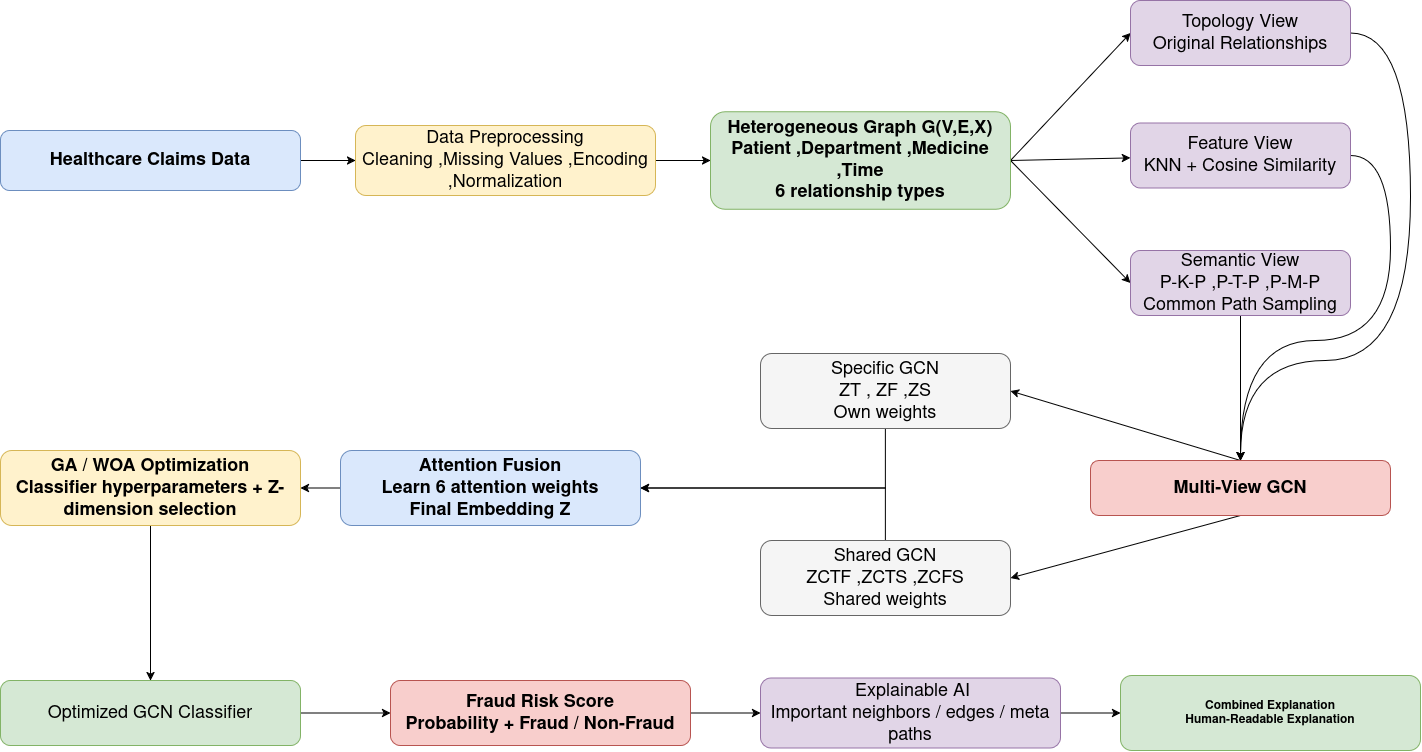
\includegraphics[
    width=0.95\paperwidth,
    height=0.72\paperheight,
    keepaspectratio
]{methodology.png}

\vfill

\end{frame}


\begin{frame}{Expected Timeline}

\centering
\scriptsize

\begin{tabular}{p{0.22\textwidth}p{0.22\textwidth}p{0.22\textwidth}p{0.22\textwidth}}
\toprule

\textbf{Review 1} &
\textbf{Review 2} &
\textbf{Review 3} &
\textbf{Final Review} \\

\midrule

\begin{itemize}
    \item Problem Identification
    \item Literature Survey
    \item Identify Research Gaps
    \item Formulate Problem Statement
    \item Identify Suitable Dataset
\end{itemize}

&

\begin{itemize}
    \item Dataset Collection
    \item Data Cleaning and Preprocessing
    \item Heterogeneous Graph Construction
    \item Construct Topology View \& Feature View \& Semantic View
     \&Multi-View GCN
    \item Initial Model Training
    \item GA/WOA Optimization
\end{itemize}

&

\begin{itemize}
    %\item GA/WOA Optimization
    \item Hyperparameter Optimization
    \item Feature/Embedding Optimization
    \item Attention Fusion
    \item Fraud Classification
    \item Explainable AI integration
    \item Generate Explanations
    \item Performance Evaluation
 
\end{itemize}

&

\begin{itemize}
    \item Final Optimized Model
    \item Complete Experimental Results
    \item Baseline Comparison
    \item Ablation Analysis
    \item XAI Results
    \item Final Conclusions
  
\end{itemize}

\\

\bottomrule
\end{tabular}

\end{frame}



\begin{frame}{References}
\scriptsize

\begin{thebibliography}{99}

\bibitem{ref1}
E. Nabrawi and A. Alanazi,
``Fraud Detection in Healthcare Insurance Claims Using Machine Learning,''
\emph{Risks}, vol. 11, no. 9, p. 160, 2023,
doi: 10.3390/risks11090160.

\bibitem{ref2}
M. Tubishat, D. Tbaishat, A. M. Al-Zoubi, A.-E. Hraiz, and M. Habib,
``Leveraging evolutionary algorithms with a dynamic weighted search space
approach for fraud detection in healthcare insurance claims,''
\emph{Knowledge-Based Systems}, vol. 317, p. 113436, 2025,
doi: 10.1016/j.knosys.2025.113436.

\bibitem{ref3}
J. Cai, S. Wu, Y. Zhang, J. Shao, and Y. Tao,
``WCGAN-GA-RF: Healthcare Fraud Detection via Generative Adversarial
Networks and Evolutionary Feature Selection,''
\emph{Information}, vol. 17, no. 4, p. 315, 2026,
doi: 10.3390/info17040315.

\bibitem{ref4}
B. Hong, P. Lu, H. Xu, J. Lu, K. Lin, and F. Yang,
``Health insurance fraud detection based on multi-channel heterogeneous
graph structure learning,''
\emph{Heliyon}, vol. 10, no. 9, p. e30045, 2024,
doi: 10.1016/j.heliyon.2024.e30045.


\bibitem{ref5}
D. Thornton, M. Brinkhuis, C. Amrit, and R. Aly,
``Categorizing and Describing the Types of Fraud in Healthcare,''
\emph{Procedia Computer Science}, vol. 64, pp. 713--720, 2015,
doi: 10.1016/j.procs.2015.08.594.

\end{thebibliography}

\end{frame}
\begin{frame}[plain]

\vfill

\begin{center}

{\Huge\bfseries Thank You}

\vspace{8mm}



\vspace{12mm}

{\normalsize
\textbf{Thirilokkiyan K}\\[2mm]
Roll No.: 206125028\\[2mm]
Guide: Dr. C. Mala\\
Professor (HAG)
}

\vspace{8mm}

{\normalsize
Department of Computer Science and Engineering\\
National Institute of Technology Tiruchirappalli
}

\end{center}

\vfill

\end{frame}
\end{document}